\documentclass{article}
\usepackage{fullpage}
\usepackage{amsmath}
\usepackage{amssymb}
\usepackage{graphicx}

\setcounter{secnumdepth}{0}
\newcommand{\emptyspace}{\{0\}}
\newcommand{\reals}{\mathbb{R}}
\newcommand{\complex}{\mathbb{C}}
\newcommand{\trace}{\textrm{tr}}
\begin{document}

\begin{center}CIS 515 --- HW4\\Sam Panzer and Kevin Shi\end{center}
\subsection{Problem B1}
\subsubsection{(1)}
Set $m=$ argmin$_i \, |(Av)_i|$ and $n=$ argmin$_i \, |v_i|$. Assume for the sake of contradiction that we have
 \[v_n \delta > (Av)_m = \displaystyle\sum_jA_{jm}v_j\]

Now consider $(Av)_n=\displaystyle\sum_{j\neq n}A_{jn}v_j+A_{nn}v_n$. By diagonal dominance we know that the last term determines the sign of the overall sum, so thus this is minimized by
\[\displaystyle\sum_{j\neq n}A_{jn}v_j+A_{nn}v_n \ge |A_{nn}||v_n| - \displaystyle\sum_{j\neq n} |A_{jn}||v_j| = \]

Now $v_n \ge v_j \, \forall \, j$, so this becomes
\[\ge |A_{nn}||v_n| - \displaystyle\sum_{j\neq n} |A_{jn}||v_n|=|v_n|\left(|A_{nn}|-\displaystyle\sum_{j\neq n}|A_{jn}|\right)\]

But we have 
\[\delta = \min \left(|A_{ii}|-\displaystyle\sum_{j\neq i}|A_ji|\right)\]

so thus
\[|v_n|\left(|A_{nn}|-\displaystyle\sum_{j\neq n}|A_{jn}|\right) \ge |v_n|\delta > (Av)_m\]
this is a contradiction since $m$ was supposed to maximize the quantity. So $\|v\|_{\infty}\delta \le \|Av\|_{\infty}$
\subsubsection{(2)}
Suppose we had
\[\displaystyle\sup_{v\neq 0}\dfrac{\|A^{-1}v\|_{\infty}}{\|v\|_{\infty}} > \displaystyle\sup_{w\neq 0}\dfrac{\|w\|_{\infty}}{\|Aw\|_{\infty}}\]
then choose $w=A^{-1}v$ where $v$ is the maximizing argument of the LHS, so 
\[\dfrac{\|w\|_\infty}{\|Aw\|_{\infty}}=\dfrac{\|A^{-1}v\|_{\infty}}{\|AA^{-1}v\|_{\infty}}=\dfrac{\|A^{-1}v\|_{\infty}}{\|v\|_{\infty}} > \displaystyle\sup_{w\neq 0}\dfrac{\|w\|_{\infty}}{\|Aw\|_{\infty}}\]
which is clearly a contradiction. Similarly if
\[\displaystyle\sup_{v\neq 0}\dfrac{\|A^{-1}v\|_{\infty}}{\|v\|_{\infty}} < \displaystyle\sup_{w\neq 0}\dfrac{\|w\|_{\infty}}{\|Aw\|_{\infty}}\]
then choose $v=Aw$ where $w$ is the maximizing argument of the RHS to get
\[\dfrac{\|A^{-1}v\|_{\infty}}{\|v\|_{\infty}} = \dfrac{\|A^{-1}v\|_{\infty}}{\|v\|_{\infty}} > \displaystyle\sup_{v\neq 0}\dfrac{\|A^{-1}v\|_{\infty}}{\|v\|_{\infty}}\]
which is again a contradiction. So the two have to be equal.

\subsection{Problem B2}
\subsubsection{(1)}
Given $A \in GL_n$ and $||\cdot||$ a vector norm on $\complex^n$, we need to show
three properties:
\begin{itemize}
  \item For any $x \in \complex^n, ||x||_A \geq 0$ and $||x||_A = 0$ iff $x = 0$.\\
    $||x||_A = ||Ax||$, whose nonnegativity is inherited from $||\cdot||$.
    Additionally, $||Ax||$ is zero iff $Ax = 0$, and $Ax = 0$ iff $x = 0$ because $A$ is invertible.
  \item $||\lambda x||_A = |\lambda|||x||_A$, for all $x \in \complex^n, \lambda \in \complex$.\\
    $||\lambda x||_A = ||\lambda A x|| = |\lambda|||A x|| = |\lambda| ||x||_A$, since 
    $||\lambda A x|| = |\lambda|||A x||$ from $||\cdot||$.
  \item For any $x,y \in \complex^n, ||x+y||_A \leq ||x||_A + ||y||_A$.\\
    $||x+y||_A = ||A(x+y)|| = ||Ax + Ay|| \leq ||Ax|| + ||Ay|| = ||x||_A + ||y||_A$.
\end{itemize}

\subsubsection{(2)}
This time, $A \in GL_n$ and $B \in M_n$. By definition, 
$||B||_A = ||ABA^{-1}|| = \displaystyle{\sup_{x \in \complex^n, ||x|| = 1}} ||ABA^{-1}x||$
\begin{itemize}
  \item $||B||_A \geq 0$ and $||B||_A = 0$ iff $B = 0$. \\
    Nonnegativity is obvious, since we're taking the sup of the norm of vectors, and these norms must
    be nonnegative. When $B = 0, ABA^{-1}x$ is clearly $0$ for any $x$, and if $B \neq 0$,
    then $ABA^{-1}$, which has the same rank as $B$, must be nonzero.
    So at least the $x$ that is all zeros except for a 1 in a column where $ABA^{-1}$ has
    some nonzero entry will yield $||ABA^{-1}x|| > 0$, which means the sup is positive.
  \item $||\lambda B||_A = |\lambda|||B||_A$.\\
    Well, $||\lambda B||_A = ||A\lambda BA^{-1}|| = |\lambda|||ABA^{-1}|| = |\lambda|||B||_A$.
  \item For any $B, C \in M_n, ||B + C||_A \leq ||B||_A + ||C||_A$.\\
    $||B + C||_A = ||A(B + C)A^{-1}|| = ||ABA^{-1} + ACA^{-1}|| \leq ||ABA^{-1}|| + ||ACA^{-1}||
     \leq ||B||_A + ||C||_A$.
  \item And finally, $||BC||_A \leq ||B||_A||C||_A$.\\
    $||BC||_A = ||ABCA^{-1}|| = ||ABA^{-1}ACA^{-1}|| \leq ||ABA^{-1}||||ACA^{-1}|| = ||B||_A||C||_A$

\end{itemize}

\subsection{Problem B3}
\subsubsection{(1,2)} This is part of the code submission!
\subsubsection{(3,4)}
It's not hard to come up with this. We generated the matrix using exactly two vectors:
$u = (1,2,3,\dots,n)$ and $v = (1,1,\dots,1)$. Clearly, row $i$ is equal to $u + (i-1)v$.
Since $u$ and $v$ are linearly independent, $A$ has rank $2$.

In particular, this tells us that subtracting row $i$ from row $i+1$ will turn row $i+1$ into $v$.
If we do this once for each $i$ from $n-1$ to $1$, we are left with a matrix that has $u$
for its first row and $v$ for all the other rows.
Subtracting row $2$ from all rows below it therefore zeros out the matrix, giving us
\[
R = \left(
\begin{array}{ccccc}
1 & 2 & 3 & \dots & n\\
1 & 1 & 1 & \dots & 1\\
0 & 0 & 0 & \dots & 0\\
\vdots & \vdots & \vdots & \ddots & \vdots\\
0 & 0 & 0 & \dots & 0
\end{array}
\right)
\]
Which clearly reduces to the desired form after subtracting row 2 from row 1 (but we think this is prettier!

\subsection{Problem B4}
The characteristic polynomial of $A$ is $|\lambda I - A|$, which is equal to 
\[
\left|
\begin{array}{ccccc}
\lambda - 1 & -2 & -3 & \dots & -n\\
-2 & \lambda - 3 & -4 & \dots & -(n+1)\\
-3 & -4 & \lambda -5 & \dots & -(n+2)\\
\vdots & \vdots & \vdots & \ddots & \vdots\\
-(n-1) & -n & -(n+1) & \dots & -2n\\
-n & -(n+1) & -(n+2) & \dots & \lambda -(2n + 1)
\end{array}
\right|
\]
Note that row $i$ is initially equal to
$(-i, -(i+1),\dots,-2i + 2, \lambda - 2i +1, -2i,\dots, -(i + n))$,
where the $i^{\text{th}}$ location has the $\lambda$.
If we consider subtracting row $i$ from row $i+1$ (with $i > 1$), then we find that row $i+1$ is.
So row $i+1$, after the subtraction, is 
$(-1, -1, \dots, -1, -\lambda -1, \lambda - 1, -1, \dots, -1)$
And now we have
\[
\left|
\begin{array}{cccccc}
\lambda - 1 & -2 & -3 & \dots & -(n-1)& -n\\
-\lambda - 1 & \lambda - 1 & -1 & \dots & -1 & -1\\
-1 & -\lambda - 1 & \lambda - 1 & \dots & -1 & -1\\
\vdots & \vdots & \vdots & \ddots & \vdots & \vdots\\
-1 & -1 & -1 & \dots & \lambda -1 & -1 \\
-1 & -1 & -1 & \dots & -\lambda - 1 & \lambda -1
\end{array}
\right|
\]

Then, we subtract row $i + 1$ from row $i$ (for $3 \leq i \leq n-1)$, to get
\[
\left|
\begin{array}{cccccccc}
\lambda - 1 & -2 & -3 & -4 & \dots & -(n-1)& -n\\
-\lambda - 1 & \lambda - 1 & & -1 -1 & \dots & -1 & -1\\
-\lambda  & 2 \lambda & \lambda & 0 & \dots & 0 & 0\\
0 & -\lambda & 2\lambda & -\lambda & \dots & 0 & 0\\
\vdots & \vdots & \vdots & \vdots & \ddots & \vdots & \vdots\\
0 & 0 & 0 &  0 &\dots & 2\lambda  & -\lambda \\
0 & 0 & 0 & 0 & \dots & -\lambda & 2\lambda
\end{array}
\right|
\]

If we divide all rows after the first two by $\lambda$, then we find that 
$P_A(\lambda) = (-\lambda)^{n-2}P(\lambda)$, as desired.

\subsubsection{(2)}
We note that the sum of the roots of $P_A(\lambda)$ is the trace of $A$.
Since $P(\lambda) \lambda^{n-2} = P_A(\lambda)$, the sum of the roots of $P(\lambda)$ is equal to the sum of the roots of $P_A(\lambda)$, as $n-2$ of those roots are all 0.

So, we just need to compute the trace of $A$, which happens to be the sum of the first $n$ odd numbers.
Well, the sum of the first $n$ odd numbers is $n^2$, as can be seen by a quick inductive proof.  
The base case of $n=1$ is trivial. For the inductive step, we note that the $k^\textrm{th}$ odd number is $2k-1$ and consider 
$n^2 + (2(n+1)-1) = n^2 + 2n + 1 = (n+1)^2$.

Thus $\trace(P(\lambda)) = n^2$.

\medskip
The product of the roots of the characteristic polynomial of which $P(\lambda)$ is the determinant happens to be the determinant of the original matrix; this is one of the identities from class.
We can, of course, find the determinant of the original matrix by plugging $0$ into the characteristic polynomial, which gives us $\lambda_1\lambda_2 = P(0)$.

\subsubsection{(3)}
Following the suggestion, we look at the process described. First, we add
$-u_k$ times row 3 to row 1 and we add $v_k$ times row 3 to row 2.
After subtracting row 2 from row 1, we have
\begin{eqnarray*}
u_{k+1} &=&  x_k + 2u_k - v_{k+1} = x_k + 2u_k - (y_k + 2v_k)\\
x_{k+1} &=&  -3 - u_k - y_{k+1} = -3 - u_k - (-1 - v_k)\\
v_{k+1} &=&  y_k + 2v_k \\
y_{k+1} &=&  -1 - v_k
\end{eqnarray*}
which is equivalent to the expanded versoin of the desired form.

\subsubsection{(4)}

\subsection{Problem B5}
The requested plots. One which converges quickly $(<100)$ and one which converges slowly $(>1000)$.

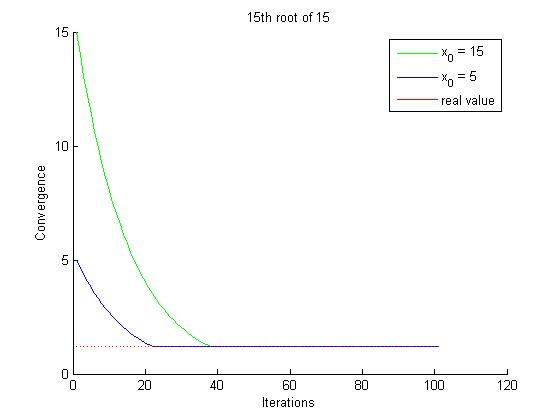
\includegraphics[height=3in, width=5in]{15rt15.jpg}

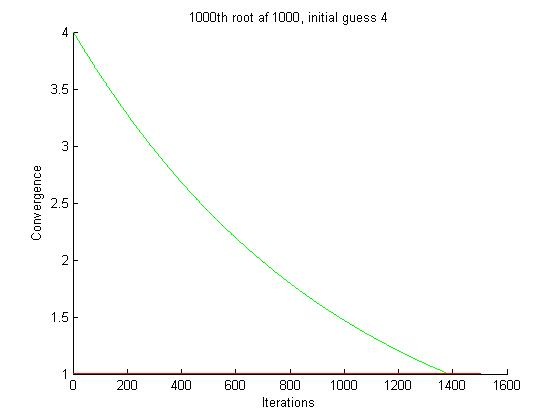
\includegraphics[height=3in, width=5in]{1000rt1000i4.jpg}


\end{document}
